\chapter*{Week 2: Variables and Operators}
\addcontentsline{toc}{chapter}{Week 2: Variables and Operators}
\setcounter{chapter}{2}
\setcounter{section}{0}

\begin{abstract}
This week you will:
\begin{enumerate}
    \item Be able to identify and understand variable types and operations on variables
    \item Implement variables and operations in a C++ program to solve a computational problem
    \item Write arithmetic expressions and assignment statements in C++
    \item Appreciate the importance of comments and good code layout
    \item Create programs that read and process input, and display the results

\end{enumerate}
    
\end{abstract}

\section{Background}
\subsection{Variables and Operators}
This week we learned about variables and basic arithmetic operators in computer science. 

Variables in computer science are similar to variables you have seen in other math and science courses. A \textbf{variable} is a value that can change, depending on conditions or on information passed to the program.

A computer stores variables differently depending on the type of information they are meant to contain, so we must declare the type of variable. This table will tell you the names of different types of variables in C++:

\begin{table}[H]
    \centering
    \begin{tabular}{c|c|c|c}\hline
         Type of variable & Declaration in C++ & Size & Description \\\hline
         Integer & int & 2 or 4 bytes & a number that has no decimal value \\
         Float & float & 4 bytes & a number that has short decimal values \\
         Double & double & 8 bytes & a number that can have longer decimals \\
         Character & char & 1 byte & stores a single letter/character using ASCII values \\
         Boolean & bool & 1 byte & stores either True or False 
    \end{tabular}
\end{table}

In order to create and use a variable, you must declare it using the appropriate declaration from the above table and then give it a name. You may also provide it an initial value, but this is not required to create a variable. Some examples include:

\begin{example}
Here is an example of declaring variables:
\begin{minted}{c++}
int myNumber = 0;
double myDecimal = 3.1415;
char myEmptyChar;
\end{minted}
\end{example}

After declaring variables, you can access them without repeating their data type. You can also perform basic operations, including the ones listed in this table:

\begin{table}[H]
    \centering
    \begin{tabular}{c|c|c}\hline
        Operator & Description & Example \\ \hline
        \mintinline{c++}{+}	& Adds together two values & \mintinline{c++}{x + y}\\
        \mintinline{c++}{+=} & Adds to itself and stores the new value& \mintinline{c++}{x += y}\\
        \mintinline{c++}{-} & Subtracts one value from another & \mintinline{c++}{x - y} \\
        \mintinline{c++}{*} &	Multiplies two values & \mintinline{c++}{x * y} \\
        \mintinline{c++}{/} & Divides one value by another & \mintinline{c++}{x / y} \\
        \mintinline{c++}{%} & Modulus; this returns the division remainder & \mintinline{c++}{x % y} \\
        \mintinline{c++}{++} & Increment; this increases the value of a variable by 1 & \mintinline{c++}{++x} \\
        \mintinline{c++}{--} & Decrement; this decreases the value of a variable by 1 & \mintinline{c++}{--x}
    \end{tabular}
\end{table}

\begin{example}
Here is an example of declaring variables and using operators:
\begin{minted}{c++}
    int myNumber = 4;
    int mySecondNumber = 5;
    int mySum = myNumber+mySecondNumber;
    int myThirdNumber = 6;
    mySum = mySum + myThirdNumber;
    int myFourthNumber = 7;
    mySum += myFourthNumber;
\end{minted}

By the end of this code, the variable \mintinline{c++}{mySum} would contain 4+5+6+7, or 22. 
\end{example}

\subsection{Characters}

Characters are a variable type that is made of a single byte, which means they can encode for a fairly limited number of characters. We can identify which characters we can store using an ASCII table shown below. 

Characters can be referred to by placing the chosen character in single quotation marks, like this:

\mintinline{c++}{char myChar = 'a';}

Characters can also can be accessed using numerical values. Since every sequence of binary numbers that encodes a character could also instead be interpreted as an integer, we can use those numbers to identify which character we are talking about. The integer values that correspond with each letter are shown in the ASCII table.

There are a few traits that you may find helpful as you move forward: firstly, observe that all lower case letters are listed in consecutive alphabetical order, and secondly that all upper case letters are similarly listed in consecutive alphabetical order. This means that the space between a lowercase `a' and a capital `A' is the same as the space between a lowercase `b' and a capital `B' and so on. This is useful for converting characters from lowercase to uppercase. 

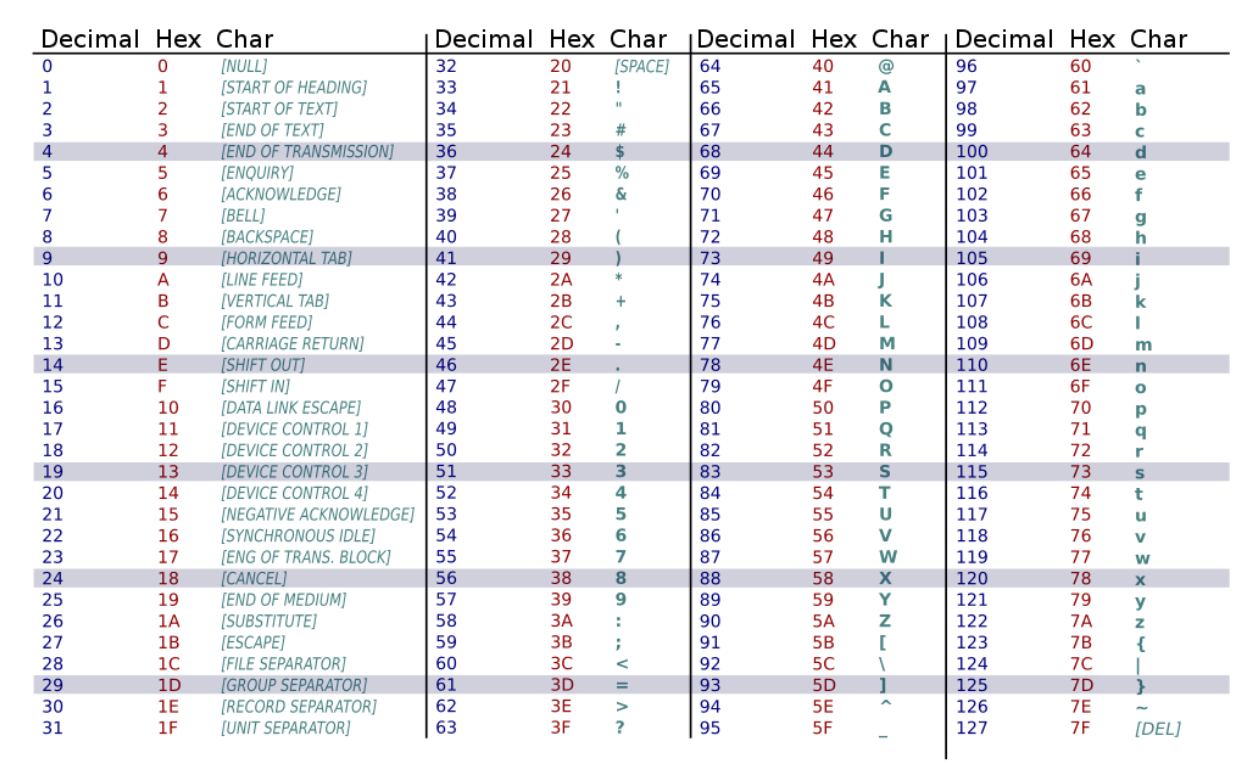
\includegraphics[width=\textwidth]{images/ascii_table.png}

\subsection{Strings}

In C++, a \mintinline{c++}{string} is a data type that represents sequences of characters instead of a numeric value (such as \mintinline{c++}{int} or \mintinline{c++}{float}). A string literal can be defined using double-quotes. So \mintinline{c++}{"Hello, world!"}, \mintinline{c++}{"3.1415"}, and \mintinline{c++}{"int i"} are all strings. We can access the character at a particular location within a string by using square brackets, which enclose an index which you can think of as the address of the character within the string. Importantly, strings in C++ are indexed starting from zero. This means that the first character in a string is located at index 0, the second character has index 1, and so on. For example:

\begin{minted}{c++}
string s = "Hello, world!";
cout << s[0] << endl;  //prints the character 'H' to the screen
cout << s[2] << endl;  //prints the character 'l' to the screen
cout << s[9] << endl;  //prints the character 'r' to the screen
cout << s[12] << endl; //prints the character '!' to the screen
    
\end{minted}

Note that when a character in a string is accessed with square brackets, the character has type char. For example:

\begin{minted}{c++}
string str = "Example"; //this is a string
char c = str[1]; //this is a char
\end{minted}

There are many useful standard functions available in C++ to manipulate strings. One of the simplest is \mintinline{c++}{length()}. We can use this function to determine the number of characters in a string. 

\begin{minted}{c++}
string s = "Hello, world!";
int s_length = s.length();
cout << s_length << endl; //This line will print 13 to the screen    
\end{minted}

Notice how the length function is called.

The correct way:

\begin{minted}{c++}
    s.length()
\end{minted}

Common incorrect ways:

\begin{minted}{c++}
    length(s)
    s.length 
\end{minted}

Another useful function available for strings is \mintinline{c++}{substr()}. This function allows us to access a subset, or a small portion, of a longer string. The substring function takes two arguments:

\begin{itemize}
    \item The starting index of the substring you would like to capture
    \item The length of the substring you would like to capture (optional)
\end{itemize}

Note that the second argument is optional. If you don't pass a second argument to subtring, then the function will print the entirety of the string, beginning with the character at the position specified in the first argument. Note that \mintinline{c++}{substr()} always returns a variable of type \mintinline{c++}{string}, regardless of the length of the substring.

For example, consider the code below:

\begin{example}
    Substring example code:

\begin{minted}{c++}
string str = "Coding is fun!";
cout << str.substr(0, 6) << endl;
cout << str.substr(6) << endl;
cout << str.substr(1, 1) << endl; //prints a string of length one
\end{minted}
\end{example}

This will ouput the following:

\begin{minted}{c++}
Coding
 is fun!
o
\end{minted}


Note: The second line of output begins with a space.

Both \mintinline{c++}{length()} and \mintinline{c++}{substr()} are special kinds of functions associated with objects, usually called methods, which we will discuss later in the course.

\subsection{Terminal Input and Output}

It is important to be able to take input from the user or to print output to the terminal as your program runs. You can do this using \mintinline{c++}{cin} and \mintinline{c++}{cout} for input and output, respectively. 

The Hello World program you have seen provides an example of using \mintinline{c++}{cout} to display output.

\begin{example}
Hello World for C++:
\begin{minted}{c++}
    #include <iostream>

    using namespace std;

    int main() {
        cout << "Hello, world!" << endl;
        
        return 0;
    }
\end{minted}

\end{example}

You can similarly ask the user for a particular value and store that value in a variable using \mintinline{c++}{cin}:

\begin{example}
An example of collecting user input to sum two integer variables and then printing their sum
\begin{minted}{c++}
    #include <iostream>

    using namespace std;

    int main() {
        int firstNum;
        int secondNum;
        cout << "Please provide one number:" << endl;
        cin >> firstNum;
        cout << "Please provide a second number:" << endl;
        cin >> secondNum;
        cout << "The sum of these two numbers is " << firstNum + secondNum << endl;

        return 0;
    }
\end{minted}

\end{example}

\subsection{Pseudocode and Algorithms}

Pseudocode is used to develop algorithms. An algorithm is a procedure for solving a problem.

An algorithm describes actions to be executed and the order in which those actions are to be executed. In other words, an algorithm is merely the sequence of steps taken to solve a problem; like a recipe. An algorithm is not computer code. Algorithms are just the instructions which provide a clear path for you to write the computer code.

\begin{example}
    An algorithm for adding two numbers together:

Step 1: Start

Step 2: Declare variables num1, num2, and sum.

Step 3: Read values num1 and num2.

Step 4: Add num1 and num2 and assign the result to sum.

Step 5: Display sum

Step 6: Stop
\end{example}

The main difference between an algorithm and pseudocode is that an algorithm is a step by step procedure to solve a given problem while pseudocode is a method of writing an algorithm. In other words, an algorithm is how to solve a problem while pseudocode is how to implement that solution. 

\begin{table}[H]
    \centering
    \begin{tabular}{p{3 in}|p{3 in}} \hline 
    Algorithm 	& Pseudocode \\ \hline
An unambiguous specification of how to solve a problem. & An informal high-level description of the operating principle of a computer program or other algorithm. \\ \hline
Helps to simplify and understand the problem. & A method of developing an algorithm. \\\hline
    \end{tabular}
\end{table}

Pseudocode is informal language that helps programmers develop algorithms (or recipes). Although there are no hard and fast rules for pseudocode, there are some suggestions to help make pseudocode more understandable and easy to read.

For instance, consider indenting all statements showing a ``dependency”, like statements that use: While, do, for, if.

Several keywords are often used to indicate common input, output, and processing operations.

\begin{table}[H]
    \centering
    \begin{tabular}{c|c}
    Input:	& READ, OBTAIN, GET \\
    Output:	& PRINT, DISPLAY, SHOW \\
    Compute: & COMPUTE, CALCULATE, DETERMINE \\
    Initialize:	& SET, INITIALIZE \\
    Add one: & INCREMENT, BUMP \\
    \end{tabular}
\end{table}

For looping and selection, the keywords that you might consider writing include:
\begin{itemize}
    \item Do While...
    \item Do Until...
    \item Case...
    \item If… then...
    \item Call ... with (parameters)
    \item Call
    \item Return ....
    \item Return
    \item When
\end{itemize}

Try to indicate the end of loops and iteration by using scope terminators.
For instance use if… (statements) ... endif.

Other words you may find useful while writing pseudocode include: Generate, Compute, Process, set, reset, increment, compute, calculate, add, sum, multiply, subtract, divide, print, display, input, output, edit, test, etc.

Be sure to indent if the indentation fosters understanding. Being clear is the purpose of pseudocode, and a very desirable goal to strive for.

Here are some examples of pseudocode:

\begin{example} Will a grade pass?
\begin{minted}{c++}
If students grade is higher than or equal to 60
	Then Print, "Passed"
else
	Print, "Failed"
\end{minted}
    
\end{example}

\begin{example} How do you find the area of a rectangle?
\begin{minted}{c++}
Read the length of the rectangle
Read the width of the rectangle
Compute the area of the rectangle as length times width.
\end{minted}
    
\end{example}

You should write pseudocode whenever you are addressing problems in computer science. This allows you space to determine how to solve a problem without worrying about syntax and formatting, instead of having to figure out everything all at once. 

\section{PreQuiz}
\begin{problem}
    What is a variable?
\end{problem}

\vspace{2cm}

\begin{problem}
    You're tracking the temperature changes throughout the day in your city. What would be a good name for this variable?
\end{problem}

\vspace{1.5cm}

\begin{problem}
    Consider a variable that represents the outcome of spinning a 6-sided spinner. What possible values could this variable hold? 
\end{problem}

\vspace{1.5cm}

\begin{problem}
    Consider a variable that tracks the distance traveled by a car in kilometers. What data type should you use? Are there multiple types that would work?
\end{problem}

\vspace{1.5cm}

\section{Recitation}

\subsection{Hello, Name!}
You have recently learned how to accept user input and store it in a variable. Write a program where you ask the user for their name in the terminal, and then print \mintinline{c++}{Hello, [name]!} in the terminal. You may find it helpful to start with the Hello World program from recitation. 

A few example runs are shown below. In these examples, red text represents user-provided text (or text you would have to type in the terminal while running the program). 

\begin{sample}
What is your name?

\textcolor{red}{Mike}

Hello, Mike!
\end{sample}

\begin{sample}
What is your name?

\textcolor{red}{samantha}

Hello, samantha!
\end{sample}

\begin{multipart}
    What steps would your program need to follow? Write these steps below.
\end{multipart}

\vspace{6cm}

\begin{multipart}
    Assume you have stored the user's name in a string variable called \mintinline{c++}{name}. How would you write the cout statement to print \mintinline{c++}{Hello, [name]!}?
\end{multipart}

\vspace{3cm}

\begin{multipart}
    Write out the steps above as a complete C++ program. Test your code. Does it work as expected? Keep testing until it does. 
\end{multipart}

\subsection{Converting Minutes to Days, Hours, Minutes, and Seconds for a Book Checkout System}
Imagine you are managing a book collection system that tracks the number of minutes a book has been checked out. You need to convert this time into days, hours, minutes, and seconds for easy display. Given a number of minutes in the range of 0 to 50,000 minutes, your program should convert this into a readable format. For example, 3,000 minutes is 2 days, 2 hours, 0 minutes, and 0 seconds.

Your program should accept user input for the number of minutes and then use that number in your calculations. Format your output as follows: 

\mintinline{c++}{The time is W days, X hours, Y minutes, and Z seconds.}

\begin{multipart}
    Explicitly list the variables you will need and their data types. 
\end{multipart}

\vspace{3cm}

\begin{multipart}
    What arithmetic operators will be most useful for this problem?
\end{multipart}

\vspace{2cm}

\begin{multipart}
    Write out the steps you would use to solve this problem by hand as pseudocode. 
\end{multipart}

\vspace{5cm}

\begin{multipart}
    Pick a random number between 0 and 50,000 for a sample run. Follow the steps you wrote from part c for this number to find your end result, and verify it. You can use your calculator, but make sure to write out each step.
\end{multipart}

\vspace{7cm}

\begin{multipart}
    Translate your pseudocode into a c++ program to solve the above code. 
\end{multipart}

\section{Homework}
\subsection{Identify and Correct the Errors}
There are several snippets of code below where there is one error. You will need to identify and correct the error so that the code compiles. This code is also available directly in CodeRunner. 

\begin{multipart}
Spot the error:

    \begin{minted}{c++}
#include <iostream> 
using namespace std;

int Main()
{
    cout << "Hello, World!" << endl;
    return 0; 
}
    \end{minted}
\end{multipart}

\begin{multipart}
Spot the error:

    \begin{minted}{c++}
#include <iostream> 
using namespace std;

int main 
{
    cout << "Hello, World!" << endl;
    return 0; 
}
    \end{minted}
\end{multipart}

\begin{multipart}
Spot the error:

    \begin{minted}{c++}
#include <iostream> 
using namespace std;

int main() 
{
    cout << "Hello, World! << endl;
    return 0; 
} 
    \end{minted}
\end{multipart}

\begin{multipart}
Spot the error:

    \begin{minted}{c++}
#include <IOstream> 
using namespace std;

int main() 
{
    cout << "Hello, World!" << endl
    return 0; 
} 
    \end{minted}
\end{multipart}

\begin{multipart}
Spot the error:

    \begin{minted}{c++}
#include <iostream> 
using namespace;
int main() 
{
    cout << "Hello, World!" < endl; 
}
    \end{minted}
\end{multipart}

\subsection{Fahrenheit to Celsius Converter}

Create a program that convert temperatures from Fahrenheit to Celsius.

$$Celsius = (Fahrenheit - 32) * (5.0 / 9.0)$$

The answer-box in coderunner is pre-loaded with following solution template for this question.

\begin{minted}{c++}
#include <iostream>

using namespace std;

int main(){
    // declare all the variable
    double fahrenheit, celsius;

    // prompt the user & get their input
    cout << "<add question>" << endl; // EDIT THIS LINE TO PROMPT USER
    cin >> fahrenheit;

    // temperature calculation
    celsius = <add equation>; // EDIT THIS LINE TO CALCULATE TEMPERATURE
    // hint: use (5.0/9.0) instead of (5/9)

    cout << "The temperature is " << celsius << " degree Celsius." << endl;
    return 0;
}
\end{minted}

Here are a few sample runs of the program, with user input shown in red:

\begin{sample}
What is the temperature in Fahrenheit? 

\textcolor{red}{32}

The temperature is 0 degree Celsius.
\end{sample}

\subsection{Calculate the Falling Time of an Object}

Create a program that calculates the time for a falling object to hit the ground based on the height from which the object fell. The equation for this is:

$$time = \sqrt{\frac{(2*height)}{9.8}}$$

\begin{itemize}
    \item \textbf{time} is the amount of time the object fell in seconds.
    \item \textbf{height} is the height the object was dropped from in meters.
\end{itemize}

\textbf{Hint:} cmath library contains a square root function that you can utilize. 

You should print the time to two decimal places. You can accomplish this by using the iomanip library and the setprecision function. Here is a sample run of the program:

\begin{sample}
How far did the object fall in meters?

\textcolor{red}{4}

The object fell for 0.90 seconds.
\end{sample}

\subsection{Volume Of A garden bed}
Write a program that calculates the amount of soil needed to fill a rectangular garden bed. Ask the user for three values: the length, width, and depth of the garden bed in inches. Use these values to calculate the total volume of the garden bed in cubic inches. Then, convert cubic inches into cubic yards and tell the user how many cubic yards of soil are needed. Print this amount to one decimal place..

\textbf{Hint:} 1 cubic inch 0.00002143 cubic yards.


\begin{sample}
What is the length of the garden bed in inches?

\textcolor{red}{20}

What is the width of the garden bed in inches?

\textcolor{red}{20}

What is the height of the garden bed in inches?

\textcolor{red}{20}

This garden bed requires 0.5 cubic yards of soil.

\end{sample}

\subsection{Water leak}
You’re managing a garden with a water tank that has a minor leak. The tank currently has some water and needs to be refilled. However, due to the leak, the water level decreases slightly every hour at a constant rate. Write a program that takes the number of hours as input (as an integer) and predicts the garden’s water level over time..

\begin{table}[H]
    \centering
    \begin{tabular}{|p{1 in}|p{1.5 in}|p{1.5 in}|p{1.5 in}|} \hline
    \textbf{Pool} & \textbf{Initial water level (Gallons)} & \textbf{Fill rate (Gallons/hour)} & \textbf{Leakage rate (Gallons/hour)} \\ \hline
    Tank A & 100 & 5.0 & 2 \\ \hline
    Tank B & 80 & 3.0 & 1.5 \\ \hline
    \end{tabular}
\end{table}

\begin{sample}
How many hours have passed?

\textcolor{red}{6}

The Garden Tank A has 112.0 gallons of water and the Garden Tank B has 87.0 gallons of water.

\end{sample}

\subsection{Barter System}
Bartering is the exchange of goods and services between two or more parties without the use of money. Below is the table of conversion values:

\begin{table}[H]
    \centering
    \begin{tabular}{|p{1 in}|p{1 in}|} \hline
    \textbf{Items} & \textbf{Values} \\ \hline
    1 bag of rice & 5 can of beans \\ \hline
    1 can of beans & 3 bottles of juice \\ \hline
    1 bottle of juice & 4 packagaes of pasta \\ \hline
    \end{tabular}
\end{table}

1 bag of rice is equal to 5 cans of beans, 1 can of beans is equal to 3 bottles of juice, and 1 bottle of juice is equal to 2 packages of pasta.

Your program should take the number of packages of pasta as input (integer) and convert its value to the maximum number of bags of rice, cans of beans, bottles of juice, and packages of pasta that can be obtained.

\begin{sample}
Enter the number of packages of pasta:

\textcolor{red}{12}

Maximum number of rice 3, beans 15, juice 45, pasta 0

\end{sample}
